\section{Building Information Modeling}
\label{sec:chapter_1_section_1}
\noindent


Una tendenza a minimizzare l'umanizzazione di nuovi territori e di spingere per il riutilizzo di alloggi
gi\'a costruiti, caduti in disuso \`e diventata una necessit\'a pressante nelle societ\'a avanzate.
Noi abbiamo intrato il modello ``zero energy'' (ogni costruzione \'e stata prodotta con il consumo della stessa energia)
con il modello ``zero waste'', ad esempio \'e un nuovo paradigma di progettazione dove i materiali di riufito della demolizione
diventano risorse per ricostruire\cite{altamura:12}.
I processi di costruizione, contrato, e progettazione necessitano di essere rinnovati per tener conto delle preoccupazioni
ambientali. Per ridurre l'impatto dei progetti di costruzione sull' ambiente, il progetto ha bisogno di prendere in
considerazione la questione dei materiali di costruzione.
Le amministrazioni pubbliche hanno bisogno di strumenti adeguati per il calcolo e il controllo dei materiali riutilizzati o smaltiti.
I nuovi strumenti dovrebbero gestire l'elaborazione digitale dei materiali in tutto il ciclo di vita del progetto,
supportando i requisiti del nuovo processo come: progettazione per Demolizione, Progettazione per il Riciclo e per i Rifiuti.
In particolare, un ciclo di vita dell'edificio, sostenuto da un processo di costruzione che prevede cicli allineati
ai fenomeni naturali è al centro di questo documento.
In questo lavoro proponiamo soluzioni che servono a chiudere il cerchio del ciclo di vita dell'edificio, allontanandosi
dalla tradizionale risposta lineare con tassi di energia ad alto consumo (dalla culla alla tomba) e verso il riutilizzo
dei materiali in decostruzione / ricostruzione (dalla culla alla culla),
supportato da computer aided processo di demolizione selettiva.
Tutti i cicli di ristrutturazione deglii edifici dovrebbero prevedere passi di de-costruzione e ri-costruzione, mirati
verso la sostituzione dei materiali al fine di ottenere una maggiore efficienza. Il trattamento di questi materiali
richiede la codifica appropriata sia per lo smaltimento, secondo il CAE (Catalogo europeo dei rifiuti) codici,
e per la pianificazione e la progettazione di nuovi edifici, seguendo la metodologia BIM (Building Information Modeling).
A questo scopo abbiamo bisogno di scene georeferenziati di realtà aumentata sulla base di modelli 3D veloci,
facilmente navigabile e misurabili.
Abbiamo già un'ottima conoscenza sui costi di costruzione (da zero), ma poco si sa circa i tassi di sostituzione
(Completare la demolizione selettiva). Un moderno processo di demolizione selettiva richiede l'intervento umano,
con costi assicurativi elevati a causa della pericolosità per coloro che lavorano in queste attività.
Quest'ultimo punto richiede un'alternativa alla sforzo umano in questi processi. Suggeriamo che i robot automatici
potrebbero sostituire sforzo umano; droni potrebbero operare in un semanticamente
contesto familiare e dare aggiornamenti in tempo reale come la realtà Contestualmente modifiche.
Riteniamo, quindi, che c'è un grande bisogno di un moderno e facile framework di modellazione da usare per la
costruzione/decostruzione nel settore AEC (Architecture, Engineering and Construction),
per consentire una realtà aumentata attraverso il riconoscimento semantico da computer vision e
fotogrammetrico di precisione fino a definizione centimetrica.
Tali strumenti di realtà virtuale / aumentata
richiedono sia veloce modellazione costruzione 3D e aumento di contenuto semantico, per poter essere controllata vicino
realtime: questa è la vera sfida richiesta anche dal futuro sviluppo di sistemi IoT.

% In questa sezione abbiamo discusso la motivazione del progetto descritto in questo documento. Le sezioni rimanenti
% sono organizzate come segue.
% Decostruction introduce un punto di vista più tecnico sullo stato di argomenti decostruzione in Europa e in Italia.
% Application descrive l'applicazione client e il flusso di lavoro proposto per geometri.
% Architecture mostra un quadro dell'architettura.
% Modelling ricorda brevemente la metodologia, stile di programmazione e ambiente di calcolo del nostro approccio
% di programmazione geometrica di modellazione solida.
% Nella sezione conclusione, si delineano il lavoro da fare e forniamo la nostra previsione sui possibili sviluppi.

% A tendency to minimize the humanization of new territories and to push for reusing already  built accommodation
% or accommodation which has fallen into disuse has become a pressing need in advanced societies.
% We have to integrate the ``zero energy'' model (each building has to produce the same amount of energy that it consumes)
% with the ``zero waste'' model, i.e. a new design paradigm where the waste materials from demolition become
% resources for reconstruction~\cite{altamura:12}.
% Building, contract, and design processes need to be renewed to take account of environmental concerns.
% To reduce the impact of construction projects on the environment, the design needs to take the issue of building
% materials into consideration.
% Public administrations need suitable tools for the calculation and the control of reused or disposed materials.
% The new tools should handle the digital processing of materials throughout the project
% life cycle, supporting new project requirements such as: Design for Deconstruction, Design for Recycling and Design for Waste.
% In particular, a building life cycle, underpinned by a construction process which envisages cycles aligned to natural phenomena
% is the focus of this paper.
% In this work we propose solutions that serve to close the circle of the building life-cycle, moving away from a traditional
% linear response with excessively high consumption energy rates (cradle to grave) and towards the reuse of materials in
% deconstruction/reconstruction (cradle to cradle), supported by computer aided selective demolition process.
% All restructuring cycles of buildings should envisage de-construction and re-construction steps, targeted
% towards the replacement of materials in order to achieve greater efficiency. The handling of these materials
% requires appropriate encoding both for the disposal, according to EWC (European Waste Catalogue) codes,
% and for the planning and design of new buildings, following BIM (Building Information Modeling) methodology.
% For this purpose we need geo-referenced scenes of augmented reality based on fast, easily navigable and measurable 3D models.
% We already have excellent knowledge about construction costs (from scratch) but little is known about replacement rates
% (complete selective demolition). A modern selective demolition process requires human intervention, with high insurance costs
% due to the danger involved for those working in these activities.
% This latter point demands an alternative to human effort in these process. We suggest that automated robots could replace human effort; drones could operate in a semantically
% familiar context and give real-time updates as the reality contextually changes.
% We believe, therefore, that there is a big need for modern and easy-to-use modeling frameworks for building deconstruction
% in the AEC (Architecture, Engineering and Construction) industry, to enable an augmented reality through semantic recognition
% by computer vision and by photogrammetric precision up to centimetric definition.
% Such virtual/augmented reality tools
% require both fast 3D building modeling and augmentation with semantic content, in order to be controlled in almost
% real time: this real challenge is also required by the future development of the Internet of Things.
% In this section we have discussed the motivation of the project described in this paper. The remaining sections are organized
% as follows.
% deconstruction introduces a more technical viewpoint about the state of deconstruction topics in Europe and in Italy.
% application describes the client application and the proposed workflow for quantity surveyors.
% architecture illustrates the framework architecture.
% modeling shortly recalls the methodology, programming style and computational environment of our geometric programming approach to solid modeling.
% In the conclusion section we outline the work to be done and provide our forecast about possible developments.
\newpage
\subsection{Applicazioni Desktop}

Autodesk \emph{Revit} è un programma CAD e BIM per sistemi operativi Windows, creato dalla Revit Technologies Inc. e comprato nel 2002 dalla Autodesk per 133 milioni di dollari[1], che consente la progettazione con elementi di modellazione parametrica e di disegno.
Revit negli ultimi sette anni ha subito profondi cambiamenti e miglioramenti. Prima di tutto, esso è stato modificato per poter supportare in maniera nativa i formati DWG, DXF e DWF. Inoltre, è stato migliorato in termini di velocità ed accuratezza di esecuzione dei rendering. A tal fine, nel 2008 il motore di rendering esistente, AccuRender, è stato sostituito con Mental Ray.
Tramite la parametrizzazione e la tecnologia 3D nativa è possibile impostare la concettualizzazione di architetture e forme tridimensionali. Questo nuovo paradigma comporta una rivoluzione nella percezione progettuale, poiché questa si sostanzia in termini non più cartesiani ma spaziali, con i vantaggi che questa può apportare alla progettazione[2].
Revit, come programma BIM,  (come si vede in Figura~\ref{fig:revit}) è da intendersi come un approccio più vicino alla realtà percepita dagli esseri umani.
Uno dei punti di forza di Revit è quello di poter generare con estrema facilità viste prospettiche o assonometriche, che richiederebbero notevoli sforzi nel disegno manuale; un esempio è la creazione di spaccati prospettici ombreggiati. Altra caratteristica di estrema importanza è quello di costruire il modello utilizzando elementi costruttivi, mentre in altri software analoghi la creazione delle forme è svincolata dalla funzione costruttiva e strutturale. Elemento portante di Revit è lo sfruttamento della "quarta dimensione", cioè il tempo. Si possono infatti impostare le fasi temporali: ad esempio, Stato di Fatto e Stato di Progetto. Ogni elemento del modello può essere creato in una fase e demolito in un'altra, avendo poi la possibilità di creare viste di raffronto con le opportune evidenziazioni: "Gialli e Rossi". I punti deboli del programma sono rappresentati, invece, dall'interfaccia talvolta poco intuitiva e dalla qualità dei rendering, che, pur utilizzando il motore "radiosity", non è paragonabile a quella ottenibile con software di rendering dedicati.

\begin{figure}[htbp] %  figure placement: here, top, bottom, or page
   \centering
   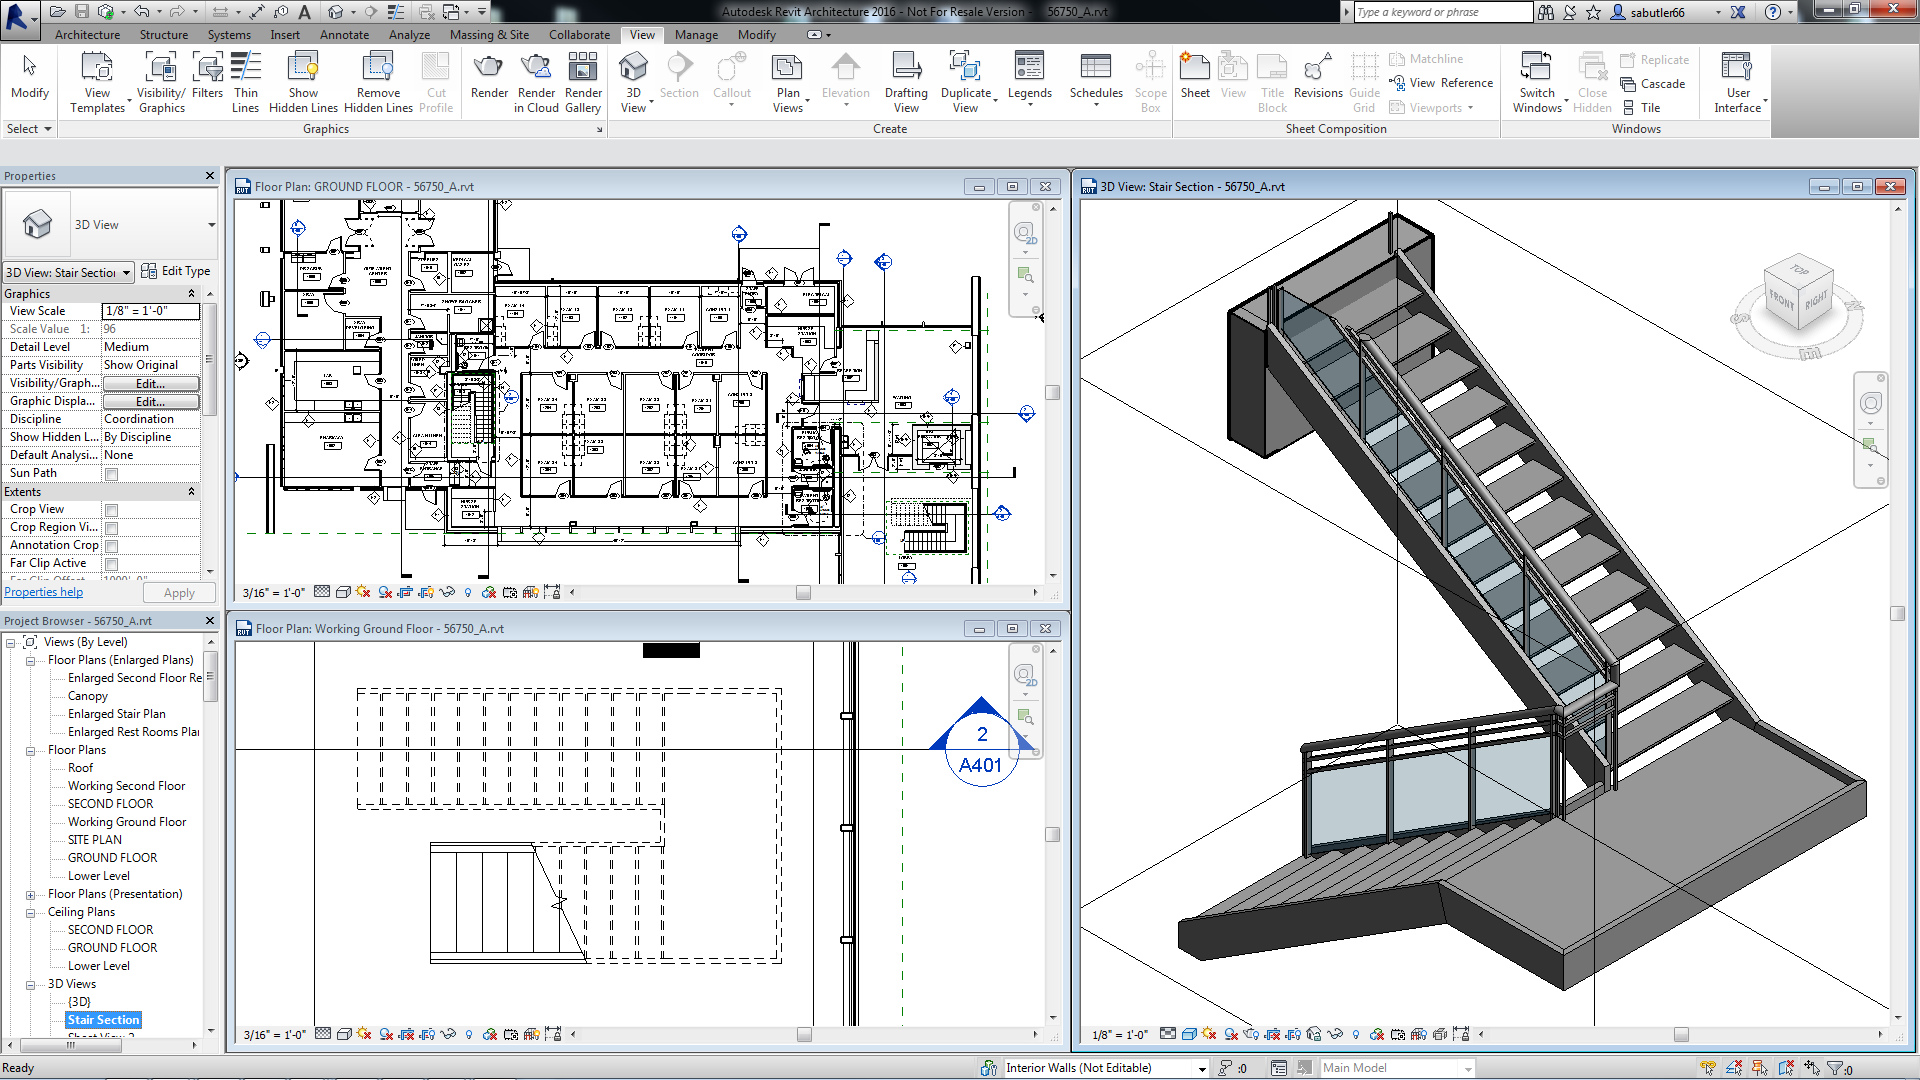
\includegraphics[width=1\linewidth]{images/revit}
   \caption{Schermata Revit}
   \label{fig:revit}
   \end{figure}
   \newpage
